\documentclass{ctexart}
\usepackage[T1]{fontenc}
\usepackage[a4paper,top=1.5cm,bottom=1.5cm,left=2cm,right=2cm,marginparwidth=1.75cm]{geometry}
\usepackage{mathtools}
\usepackage{tikz}
\usepackage{booktabs}
\usepackage{caption}
\usepackage{outlines}
\usepackage{graphicx}
\usepackage{float}
\usepackage{amsthm}
\usepackage{tabularray}
\usepackage{pdfpages}
\usepackage{minted}
\usepackage[colorlinks=false, allcolors=blue]{hyperref}
\usepackage{cleveref}
\usepackage{gbt7714}
\crefname{figure}{图}{图}
\crefname{table}{表}{表}
\bibliographystyle{gbt7714-numerical}
\UseTblrLibrary{booktabs}
\DeclarePairedDelimiter{\set}{\{}{\}}
\DeclarePairedDelimiter{\paren}{(}{)}
\graphicspath{ {./images/} }

\newcounter{fullrefcounter}
\newcommand*{\fullref}[1]{%
\addtocounter{fullrefcounter}{1}%
\label{--ref-\thefullrefcounter}%
\ifthenelse{\equal{\getpagerefnumber{--ref-\thefullrefcounter}}{\getpagerefnumber{#1}}}
  {
    \hyperref[{#1}]{\Cref*{#1} \nameref*{#1}}
  }
  {% false case
    \hyperref[{#1}]{第 \pageref*{#1} 页 \Cref*{#1} \nameref*{#1}}
  }
}
\title{基于上下文信息的汉语分词及词义消歧技术研究 \\
{\Large 自然语言处理大作业报告}}
\author{卢雨轩 19071125}
% \date{\today}
\ctexset{
    section = {
        titleformat = \raggedright,
        name = {,},
        number = \chinese{section}、
    },
    paragraph = {
        runin = false
    },
    today = small,
    figurename = 图,
    contentsname = 目录,
    tablename = 表,
}

\begin{document}

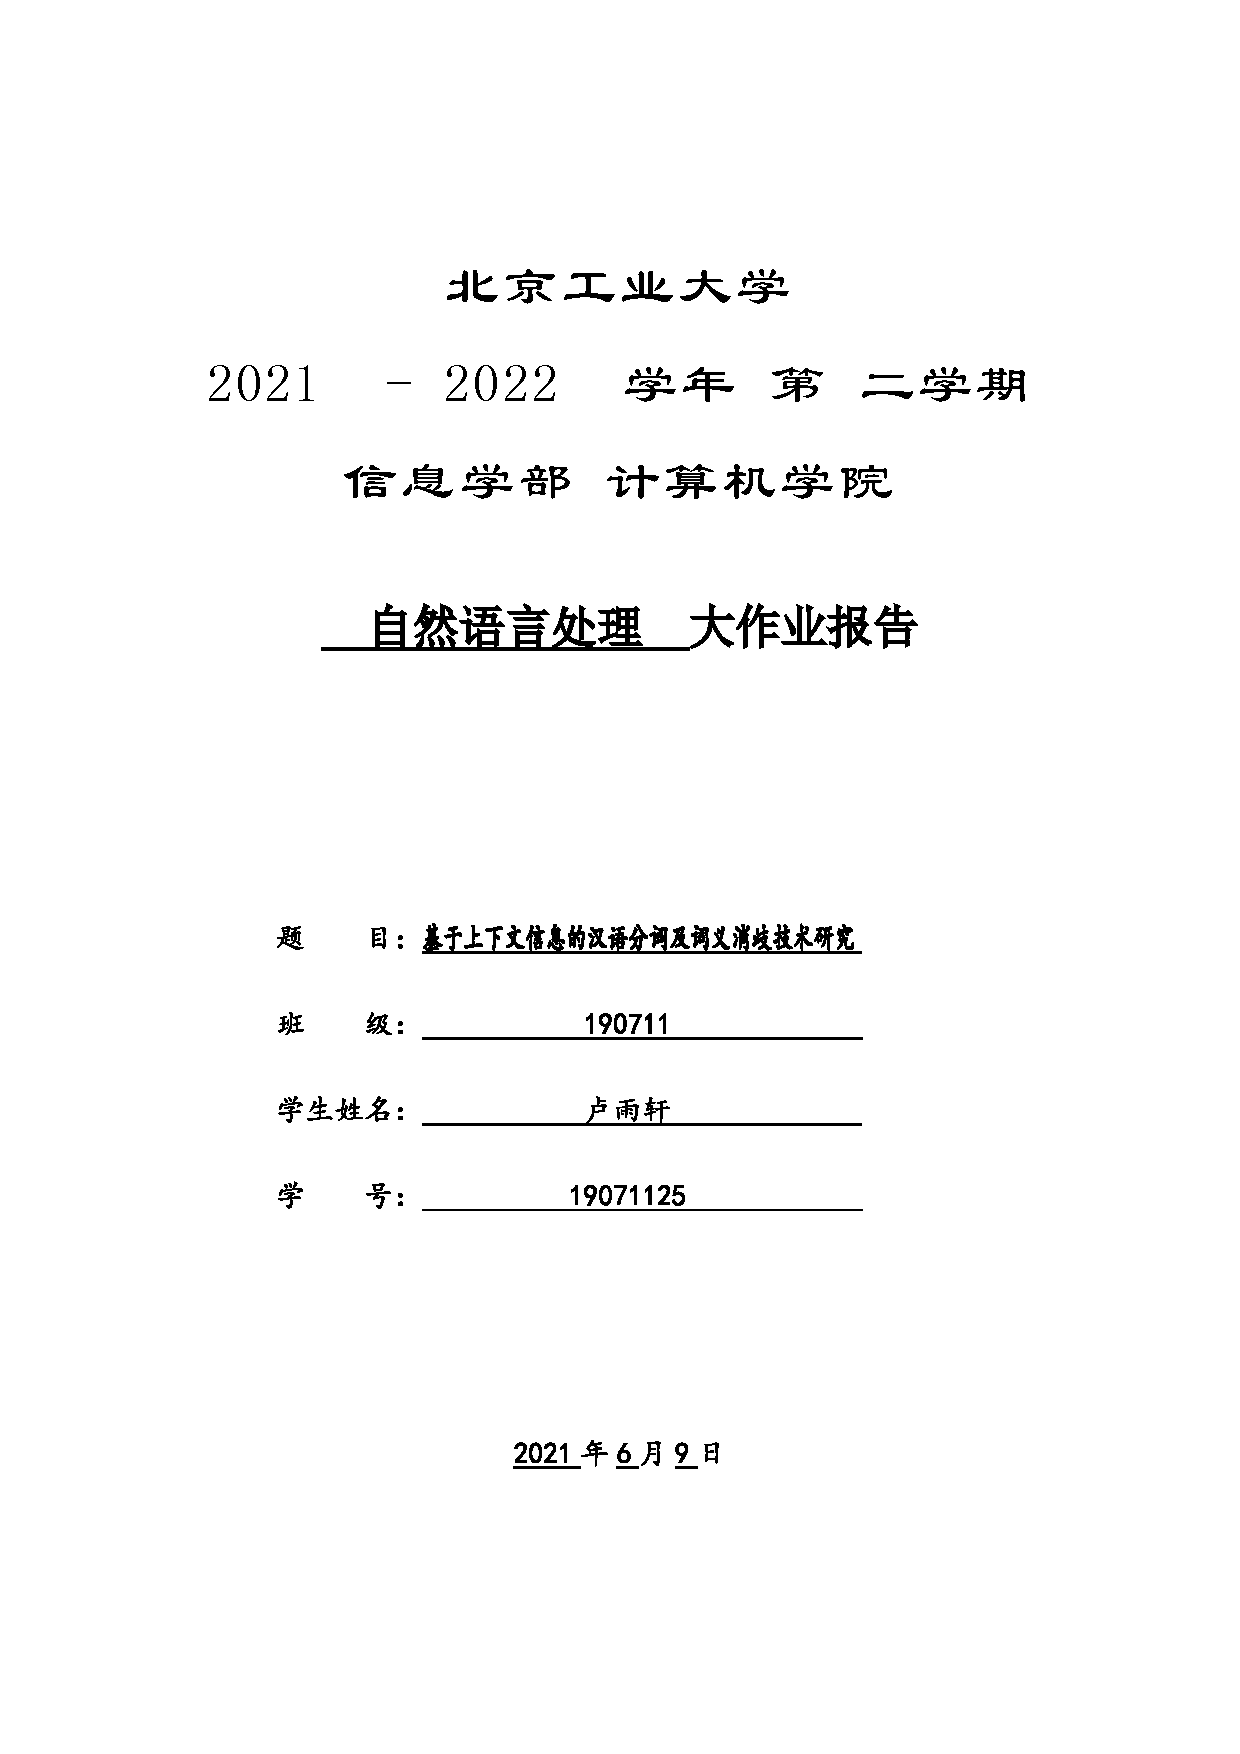
\includepdf{cover.pdf}

\maketitle

\section{介绍}

本次大作业中,我完成了一个基于上下文的汉语分词、词义消歧系统的研究,加深了我对于自然语言处理的理论知识的认知和理解。项目在微软亚洲研究院数据集上汉语分词任务中的F1值达到了 98.4\%,同SOTA模型的F1值(98.5\%)十分接近。

\section{相关工作}
汉语分词是一项NLP领域中非常传统的任务。在英语等语言中,词和词之间有明显的空格标记,但是在汉语中句子以字串的形式存在,因此对中文进行处理的第一步就是进行分词。分词的质量直接影响了下游任务的质量,是后续语义分析、文本分类等任务的基础,因此汉语分词十分重要。

传统的中文分词方法包括基于字符匹配法的分词,使用预先构建的词表对输入句子进行最大匹配。这种做法非常依赖词表的质量,也无法处理歧义问题,因此人们提出了基于统计学的分词方法。隐马尔科夫模型(HMM)应用非常广泛,通过观测值序列找到真正的银层状态层序列。最大熵隐马尔科夫模型将最大熵融入HMM中,提高了是别的精确度,召回率也大大提高。条件随机场模型通过条件概率描述模型,在考虑词频信息的同时也考虑了上下文语境信息。为了进一步提升效果,有研究人员预先手工构建同义词辞典,对同义词进行合并。但是,以上基于统计学的方法依赖于高质量的训练数据,同时也很难处理 Out-Of-Vocabulary 问题。

2005年的SIGHAN会议中给出了Bakeoff数据集,其中包括PKU、MSR两个简体中文数据集,AS、CITYU两个繁体中文数据集。高质量的数据集的发布也促进了汉语分词研究的发展,深度学习技术也开始被引入分词问题。Ma\cite{maStateoftheartChineseWord2018}等人发现使用简单的Bi-LSTM模型就可以将分词效果达到SOTA水平。Devlin\cite{devlinBERTPretrainingDeep2019}等人提出了BERT模型,创新性的提出了预训练和微调的两步训练方法,使用统一的预训练模型以高效利用大量无监督的与训练数据,经过少量微调后即可在非常多下游任务上达到SOTA。Yang\cite{yangBERTMeetsChinese2019}等人将BERT首次应用在汉语分词任务中,取得了很好的效果。Duan\cite{duanAttentionAllYou2020}等人将注意力机制应用在了汉语分词任务上,使用 Transformer 的改进模型达到了很好的结果。最近,Ke\cite{kePretrainingMetaLearning2021}等人提出了基于BERT的元学习预训练方法,使用元学习的方法同时学习多个数据集,增高了数据利用能力。

\section{基于上下文的汉语分词、词义消歧方法}

\subsection{分词算法}
我使用BERT模型后接多层感知机模型,使用BERT模型给出的基于上下文信息的 embedding 判断是否在这个字后分词。与传统方式不同的是,在我调用BERT时没有进行WordPiece分词。传统BERT会对每个词进行WordPiece分词,尽管汉语不会被分词,但是汉语中的数字(如年份等)等会被合并为一个词。这样处理对于其他下游任务可能更为有效,但是不适合汉语分词任务。因此,在我的系统中,我直接将每个字的id输入模型中,不进行WordPiece分词。

BERT模型输出的 embedding 被输入到有2个隐藏层的感知机中,感知机输出2个值,分别表示此处分词和不分词的置信度。感知机的输出值进行softmax后计算nll loss,作为训练目标:
\begin{align}
    E(I) &= Bert([CLS]; I; [SEP]) \\
    P(I) &= \mathop{tanh}(E(I) \times W_1) \times W_2 \\
    \mathcal{L}(I) &= NLL(P(I), TARGET)
\end{align}
\subsection{语义消岐方法}
我使用BERT模型输出的语义信息,随后使用K-Menas方法进行聚类、t-SNE方法进行降维,得到语义消岐的结果。

\section{实验}
\subsection{数据集}
我使用2005年的SIGHAN会议中给出的Bakeoff数据集中的MSR和PKU数据集。经过计算得到训练数据中每个汉字的信息熵为9.43,每个词的信息熵为11.1。

我对数据集进行了划分,将原先的训练集划分为训练集和验证集。划分的结果见\cref{tab:dataset}。

\begin{table}
    \centering
    \begin{tblr}{cccccc}
        \toprule
        数据集 & 字数 & 训练集(行) & 划分训练集(行) & 划分验证集(行) & 测试集(行) \\
        \midrule
        MSR & 4050566 & 86924 & 80000 & 6924 & 3985 \\
        PKU & 1826475 & 19056 & 18000 & 1056 & 1945 \\
        \bottomrule
    \end{tblr}
    \caption{数据集信息}
    \label{tab:dataset}
\end{table}


\subsection{实验环境}
我们的实验在一台AMD Ryzen 9 5950X CPU、NVIDIA GEFORCE 3090 24G的电脑上运行,使用 pytorch 1.10 作为深度学习框架。分词任务中,模型训练1个Epoch后进行验证和测试。

最终评测结果使用SIGHAN官方提供的评分脚本计算。

\subsection{实验结果}
\subsubsection{汉语分词任务}
\begin{table}
    \centering
    \begin{tblr}{cccccc}
        \toprule
        模型 & PKU & MSRA \\
        \midrule
        BERT(Yang, 2019) & 96.50 & 98.40 \\
        MetaSeg(Ke,2021) & \textbf{96.92} & \textbf{98.50} \\
        \midrule
        BERT(ours) & 95.60 & 98.40 \\
        \bottomrule
    \end{tblr}
    \caption{汉语分词任务试验结果}
    \label{tab:cws}
\end{table}
汉语分词任务的试验结果见 \cref{tab:cws}。可以看到,我们的模型基本复现了Yang\cite{yangBERTMeetsChinese2019}同样基于BERT的结果,并在MSR数据集上十分接近SOTA。
\subsubsection{语义消岐任务}
我以数据集中的『美』字为例,进行了语义消岐。消岐后各个类别的句子抽样如下:

第一类:
\begin{outline}
\1 “一个人不管学什么专业,总得懂一些文学知识,有一点艺术素养,这对于丰富自己的思想和生活,提高自己的审美能力很有好处。
\1 “传说再美丽再动听,终归是传说。
\1 “传说再美丽再动听,终归是传说。
\1 他充满自信地宣称:“美是多种多样的。
\1 如果你的一言一行都配得上她,她就会更明亮,更灿烂,更美丽。”
\1 他一笑说:“其实世界上这么多美好事物,干嘛非跟谁过不去?
\1 并且有的旧车出过事故,一经‘美容’便难以识别,这也给我们估价带来困难。”
\1 深入生活的过程,就是汲取营养的过程,就是融入时代的过程,就是寻找美、发现美、表现美的过程。”
\1 我一定会将这幅画挂在最能体现其美妙意境的地方。”
\end{outline}

第二类:
\begin{outline}
\1     二战期间,中美两国是同盟国成员,在战场上并肩战斗。
\1 影片的编剧和导演是美国人,由中美两国著名演员主演。
\1 中美合拍电影《夏日情动》已完成《夏日情动》是中美电影人共同投资拍摄的电影故事片,最近已告完成。
\1 在今天的辩论中,许多议员以大量的事实说明中国在国际事务中起着重要的积极作用,经贸关系是整个美中关系中的关键因素,并认为克林顿政府的对华接触政策符合美国利益。
\end{outline}

可以看到,模型可以有效区分『美』字的不同语义。聚类降维后结果见\cref{fig:wsd}。

\begin{figure}[h]
    \centering
    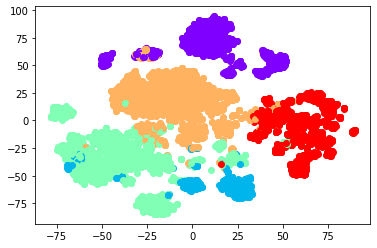
\includegraphics[width=.5\linewidth]{image1.png}
    \caption{聚类结果}
    \label{fig:wsd}
\end{figure}

\section{总结与分析}
本次实验中,我应用了BERT到汉语分词任务、词义消歧任务中。在调研相关文献的过程中,我了解了汉语分词任务的近期进展,并做出了相应实践。

在汉语分词任务上,正确率不够高主要源自BERT的512个字的长度限制。如果只统计前512个字,F1值在99.5\%左右。如果要进一步提升结果,应该考虑对于超长的句子进行适当切分,分别输入BERT并计算是否分词,应该可以显著提升效果。



\clearpage

\appendix

\bibliography{references.bib}

\end{document}
